
\documentclass{article}

\usepackage[margin=1.5in]{geometry}
\usepackage{graphicx}
\usepackage{caption}
\usepackage{float}
\usepackage[utf8]{inputenc}

\usepackage[backend=biber, style=authortitle-icomp]{biblatex}
\addbibresource{ref.bib} 
\title{
Exploration of Wetting-Dewetting Transitions of Ultra Thin Polymer Surfaces
}
\author{Raymond Sutrisno}

\begin{document}
\maketitle

\abstract{
With the increasing use of thin polymer film coatings in a variety of technological applications, there exists a need for a theoretical understanding which models the stability of these coatings with respect to some parameter space of conditions.
In this review, we introduce the reader to basic concepts of wetting phenomena, some basic concepts on the behavior of glass polymers and the nature polymeric coatings with respect to the parameter space, along with current work related to the exploration of the parameter space on dewetting ultra thin polymeric coatings.
}

\section{An Introduction to Wetting Phenomena} \label{sec1}

\subsection{Wetting Definitions}
When a liquid is placed on the surface of a substrate, the liquid evolves until it reaches a state of equilibrium. This phenomena is known as wetting.

From observations of wetting phenomena in daily life, intuition expects that liquids in a state of equilibrium tend to either spread themselves out on the surface or prefer to coalesce. From this we can define a material specific property of wettability. We say that a surface $A$ is more "wettable" than a surface $B$ with respect to a liquid $L$ if for a fixed volume of liquid $L$, the surface area of $L$ on $A$ is greater than $L$ on $B$ under the same thermodynamic conditions. The measure of wettability is conventionally quantified by the contact angle which is the angle between the liquid-atmosphere interface and the substrate, illustrated in Figure \ref{fig:contact_angle}.

\begin{figure}[H]
\caption{Illustration of characteristic contact angle $\theta$ of a liquid. When $\theta$ is zero, perfect wetting occurs whereas when $\theta$ is $180$ degrees, perfect dewetting occurs. Source : \cite{wikipediaEN:contactangleschem}}
\centering
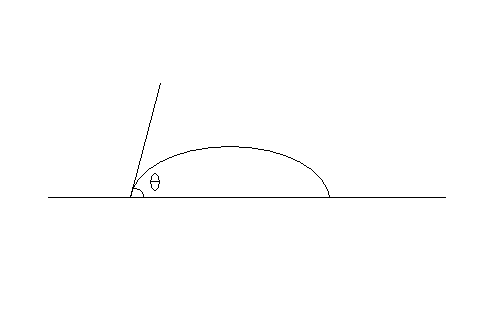
\includegraphics[width=0.5\textwidth]{./contact_angle.png}
\label{fig:contact_angle}
\end{figure}

\subsection{Intermolecular Forces and Surface Tension}
To understand why an equilibrium state exists, one must examine the intermolecular forces at play both inside the liquid (cohesive) and along the liquid-substrate interface (adhesive). In essence the cohesive forces refer to the intermolecular forces of the molecules of the liquid on one another and are responsible for the degree to which they adhere to one another. Adhesive forces are similar however focuses on the interactions between the the molecules of the liquid and the molecules of the substrate and is responsible for the degree to which the liquid molecules and substrate molecules attract one another.

Consider the cohesive forces in molecules in a liquid as in the diagram in Figure \ref{fig:cohesion_molec}. Molecules within the liquid experience equal pull from all directions whereas molecules along the surface only experience a pull inwards. This inward force, otherwise known as a surface tension, creates a pressure which causes liquids to want to minimize their surface area. It is because of this behavior that when no external forces such as gravity are present, when left to reach equilibrium, liquids prefer to rest as spheres since a sphere is the solid which minimizes the surface area to volume ratio.

\begin{figure}[H]
\caption{Diagram of cohesive forces acting on molecules of a liquid both internally and the surface.}
\centering
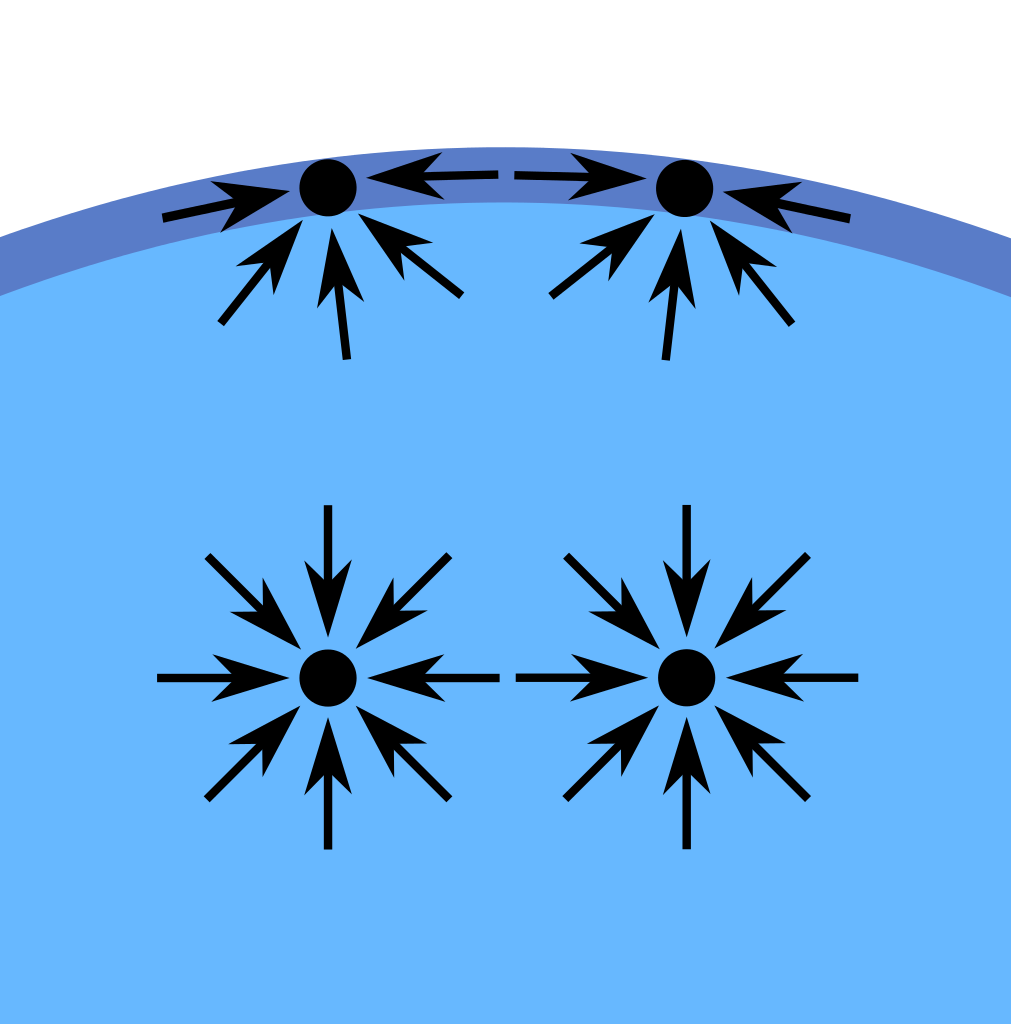
\includegraphics[width=0.4\textwidth]{./cohesion.png}
\label{fig:cohesion_molec}
\end{figure}

From this relation, a quantification of surface tension, aka surface energy, can be defined. The dimensions for this quantity are in Force per unit Length or Energy per unit Area. One intuition behind the quantification of surface tension can be thought of as the amount of force required to increase the surface area of a liquid along the direction parallel to the normal vector corresponding to the surface of that liquid. Another is the surface energy definition which can be thought of as the amount of energy required to increase the surface area by one unit. Based on the surface energy definition we can define high energy vs low energy surfaces. In materials such as metals, glasses, or ceramics, the bonding forces which bind them together (metallic, covalent, ionic) are very strong and thus the amount of energy required to break their surfaces is very high. Contrastingly low energy materials, which are characterized by weakly binding forces such as Van der Walls forces or hydrogen bonding require low amounts of energy to break their surface. 

Mathematically the relationship between surface tension and contact angle $\theta$ is modeled using the Young relation, illustrated in Figure \ref{fig:young} and equation \ref{eq:young}.

\begin{figure}[H]
\caption{Diagram depicting contact angle and Young relationship where $\gamma_{SL}$ is the surface tension along the substrate-liquid interface, $\gamma_{LG}$ is the surface tension along the liquid-gas interface, $\gamma_{SG}$ is the surface tension along the substrate-gas interface.}
\centering
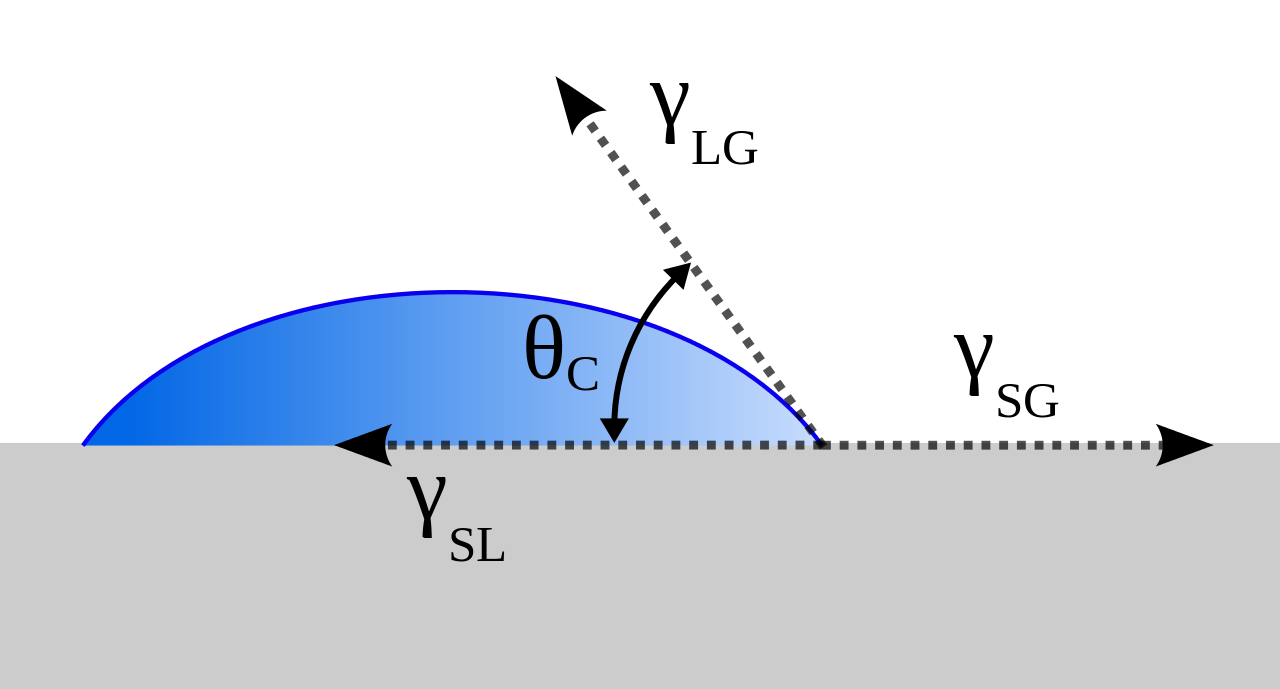
\includegraphics[width=0.5\textwidth]{./young.png}
\label{fig:young}
\end{figure}

\begin{equation} \label{eq:young}%
\mbox{\Large\( %
\gamma_{SG} = \gamma_{SL} + \gamma_{LG} cos(\theta) %
\)} %
\end{equation}

\section{Ideal Wetting of Ultra Thin Polymeric Films and Potential Sources of Dewetting}

What constitutes as ideal differs depending on use case. For most applications in industry such as photolithography etching for microfabrication, dewetting of the photomask is extremely undesirable the quality of design transfer is dependent on the uniformity of the mask. On the other hand, in nanotechnology dewetting is used as a technique to fabricate nanoparticles,\textcite{gentili2012applications}. For the purposes of this review, it is assumed that stability of these films are the desired ideal outcome.

Unlike simplified models liquid substrate systems discussed in section \ref{sec1}, there are actually two wetting agents which need to be considered in the context of polymeric coatings. These polymeric coatings are deposited on the substrate via solvent carrier. The structure of these coatings most closely resembles a mesh-like structure of physically interwoven long polymer chains which are held together by weak intermolecular forces such as Van der Walls forces and hydrogen bonding.

In order to distinguish the factors of instability of ultra thin polymeric coatings from the bulk counterparts, \textcite{ashley2005wetting} defines ultra thin polymeric coatings as coatings in which the thickness $h$ is less than an order of $100 nm$ to $ 200 nm$. According to \textcite{pahlavan2018thin}, at this level of increasing thickness the interactions at the liquid-solid and liquid-gas interface due to Van der Walls forces are much stronger in comparison to surface tension forces arising from the interactions within the liquid.



\section{Current Work in Wetting Parameter Optimization}
Much work in the area of stability exploration of the input parameter space has been limited to combinatorial studies. Papers such as \textcite{meredith2000combinatorial} and of \textcite{ashley2005wetting} are examples of these combinatorial studies on the boundaries of wetting-dewetting transitions. 


\printbibliography

\end{document}

